%-------------------------------------------------------------
% Language
% Use the option "language=EN" to set the beamer theme in English. Use
% the option "language=ES" to set the beamer theme in Spanish.

% Colors
% Use the option "color=white" to set the background in white and the
% bottom bar in blue. Use the option "color=blue" to set the
% background in blue and the bottom bar in white. Use the option
% "color=blue2" to set the background in blue and the bottom bar in
% blue.

% Font Color
% Use the option "fontc=black" to set the font color in black. If this
% argument is not given the default color is set depending of the
% color scheme selected.

% Notes:
% Do not use \large inside multicols
% Enumerate require \justifying command
% Tables captions bellow the tabular
% With citations, note = {} may only work for @misc

% Credits: https://github.com/alejogm0520 & Samuel Plazas Escudero
%-------------------------------------------------------------

%--Principal packages
\documentclass[xcolor=table, aspectratio=43,8pt, notheorems]{beamer} % 4:3; can be 16:9; [...,8pt,t] in order to start text of all frames on the upper part; add: draft to not compile figures.
\usetheme[language=EN, color=white]{EAFIT}
\usepackage[english]{babel}
\usepackage[utf8]{inputenc}
\usepackage[T1]{fontenc}
\usepackage{algorithm2e}
\usepackage{amsmath,amsfonts,amssymb,cancel}
\newcommand{\overbar}[1]{\mkern 1.5mu\overline{\mkern-0.5mu#1\mkern-0.5mu}\mkern 1.5mu}

% Equations; physics is optional and sometimes problematic!
\usepackage{verbatim} % Environments, \begin{comment}
\usepackage{fancyvrb}
%--Arial
\usepackage{helvet}\renewcommand{\familydefault}{\sfdefault}
% It's ok
%--David Plazas recommended
%\usepackage{libertine} % Normal
%--Carlos Cuartas 
%\usepackage[T1]{fontenc}\usepackage{lmodern} % Best
%--Beamer packages
\usepackage{tikz} % For making vectorized figures, arrows
\usepackage{ifthen} % For specifying conditionals for sections
\usepackage{ragged2e}\justifying % Whole text justified, except enumerate: add \justifying
\usepackage{multicol} % Multiple columns in one frame
%--Tables-Figures
\usepackage{natbib}
\usepackage{url}
\usepackage{booktabs,multirow} % Bookstyle tables
\usepackage{array} % Custom width and centered
\newcolumntype{P}[1]{>{\centering\arraybackslash}p{#1}} % horizontal centering but use custom width
\newcolumntype{M}[1]{>{\centering\arraybackslash}m{#1}} % horizontal and vertical centering but use custom width
%-Figure label
\usepackage[labelsep=period,justification=justified,format=plain]{caption} % Dot instead of colon and justified caption
%--Figure
\usepackage{graphicx,subcaption} % Figures and subfigures
\usepackage{media9} % video and audio
%-Figure-Table on top
\usepackage{float} % Allows to put H instead of ht
\setbeamertemplate{caption}[numbered] % Numbered captions
%---------TOC
\setbeamertemplate{section in toc}[sections numbered]
\setbeamertemplate{subsection in toc}[subsections numbered]
\setbeamerfont{section in toc}{size=\small}
\setbeamerfont{subsection in toc}{size=\footnotesize}
\setbeamertemplate{subsection in toc}{\leavevmode\leftskip=3.2em\rlap{\hskip-2em\inserttocsectionnumber.\inserttocsubsectionnumber}\inserttocsubsection\par} % Indented subsection
\setcounter{tocdepth}{2} % Toc depth, put 1 for only showing there the sections and 2 to include sections
%---------Cite
\usepackage{bibentry} % Full cite foot
\nobibliography* % Full cite foot
\setbeamertemplate{bibliography item}[triangle]% [online][book][article][triangle][text]; Or: \setbeamertemplate{bibliography item}{\insertbiblabel} 
\usepackage{etoolbox} % Package for using justified bibliography 
\apptocmd{\thebibliography}{\justifying}{}{} % Justified bibliography 
%---------Footnotes
\setbeamercolor{footnote}{fg=white} % Footnote white 
\setbeamercolor{footnote mark}{fg=.} % Takes the color depending on the circumpstance
\setbeamercolor{bibliography entry author}{fg=white} % Allows to have white footnote bibs
\setbeamertemplate{footnote}
{
  \hspace*{-1cm} % Horizontal movement
  \vspace*{-3.12cm} % Vertical movement
  \parbox[c][3.64cm]{10.6cm}{\tiny\noindent\insertfootnotemark\insertfootnotetext} % b: bottom, height: 3.3cm, horizontal length: 10.6cm (max horizontal)
% If there are problems, put \vspace*{-2.87cm} and \parbox[c][3.3cm]
% or \vspace*{-2.88cm} and \parbox[c][3.4cm]
% or \vspace*{-3.05cm} and \parbox[c][3.6cm]
% or \vspace*{-3.12cm} and \parbox[c][3.64cm]
}
\renewcommand{\footnoterule}{\kern -3pt \hrule width \textwidth height 0pt\kern 3pt} % No footnoterule
\usepackage{perpage}\MakePerPage{footnote} % Footnote numbered per frame
\renewcommand{\thefootnote}{\Roman{footnote}} % Roman number in footnote
                                              % Cutom: \fnsymbol{footnote}
%------------------------------------
%---------Numbered Slides and Sections
\setbox0=\hbox{\subsecname\unskip}\ifdim\wd0=0pt\else%
 ~--~\insertsubsectionhead
\fi
%------Numbering section: title in bold, centered and with a line
\newcommand{\numb} 
{
  \setbeamertemplate{frametitle}
  {
    \ifx\insertsubsection\empty % No subsection
         \bfseries\thesection.~\insertframetitle~\color{black}\par\vskip-5pt\hrulefill % \centering
    \else % subsection
         \bfseries\thesection.~\insertframetitle~\color{black}\par\vskip-9pt\hrulefill\par\vskip3pt{\large\thesection.\thesubsection~\insertframesubtitle} % Subsection with smaller size;
    \fi
  }
}
%------No numbering section: title in bold, centered and with a line
\newcommand{\nonumb}
{
  \setbeamertemplate{frametitle}{\bfseries\color{black}\centering\insertframetitle\par\vskip-6pt\hrulefill}
}
%------------------------------------
%--No hyphenation on text
\tolerance=1
\emergencystretch=\maxdimen
\hyphenpenalty=10000
\hbadness=10000
%------------------------
%---------Itemize justified in beamer
\makeatletter
\renewcommand{\itemize}[1][]{
  \beamer@ifempty{#1}{}{\def\beamer@defaultospec{#1}}
  \ifnum \@itemdepth >2\relax\@toodeep\else
    \advance\@itemdepth\@ne
    \beamer@computepref\@itemdepth % Sets \beameritemnestingprefix
    \usebeamerfont{itemize/enumerate \beameritemnestingprefix body}
    \usebeamercolor[fg]{itemize/enumerate \beameritemnestingprefix body}
    \usebeamertemplate{itemize/enumerate \beameritemnestingprefix body begin}
    \list
      {\usebeamertemplate{itemize \beameritemnestingprefix item}}
      {\def\makelabel##1{
          {
            \hss\llap{{
                \usebeamerfont*{itemize \beameritemnestingprefix item}
                \usebeamercolor[fg]{itemize \beameritemnestingprefix item}##1}}
          }
        }
      }
  \fi
  \beamer@cramped
  \justifying % Justified itemize
  \beamer@firstlineitemizeunskip
}
\makeatother
%------------------------
%---------get current section name for showing it at its begining
\usepackage{nameref}
\makeatletter
\newcommand*{\currentname}{\@currentlabelname}
\makeatother
%---------Shows in which section we are at the begining of each one
\begin{comment}
\AtBeginSection[]
{
\begin{frame}[plain,noframenumbering]
  \begin{beamercolorbox}[ht=\paperheight,wd=\paperwidth, center]{Portada}
    \begin{center}\textbf{\LARGE \currentname}\end{center} % Leave the next space mandatorily

    \vspace{0.44\paperheight}
  \end{beamercolorbox}
\end{frame}
}
\end{comment}

%---------TEXTBLOCKS-GRID 
\usepackage[absolute,overlay,showboxes]{textpos}
%\usepackage[texcoord,grid,gridunit=mm,gridcolor=red!10,subgridcolor=green!10]{eso-pic} % Helping grids, comment when publishing
%---------NOTES IN BEAMER
\AtBeginNote{\Huge}\newcommand{\notei}[1]{\note[item]{\Huge{\textcolor{blue}{#1}}}} % Use \notei{text} everywhere % [1] means one parameter located in #1 (input). 
\setbeamertemplate{note page}[plain] % Plain style for notes page
\setbeameroption{show notes} % {show notes} or {hide notes}
% \setbeameroption{show notes on second screen=right}
% as well you can use \documentclass[notes=only] at the beginning of the code
%-----------More elaborated notes
%\setbeamercolor{note page}{bg=white!90!black, fg=black}
%\setbeamercolor{note title}{bg=white!30!red, fg=black}
%\setbeamercolor{note date}{parent=note title}
%---------Itemize, enumberate and lists inside them
%\setbeamertemplate{itemize/enumerate body begin}{\LARGE} % Body
\setbeamertemplate{itemize/enumerate subbody begin}{\Large} % Subbody
%---------COLOR DEFINITIONS
\definecolor{azure(colorwheel)}{rgb}{0.0, 0.5, 1.0} % Define colors here
\definecolor{blue(ryb)}{rgb}{0.01, 0.28, 1.0}

\usepackage[normalem]{ulem}
\useunder{\uline}{\ul}{}


\usepackage{mathtools}
 \usepackage{tikz}
\DeclarePairedDelimiter{\ceil}{\lceil}{\rceil}
%%%%%%%%%%%%%%%%%%%%%%%
%Start of the Document%
%%%%%%%%%%%%%%%%%%%%%%%

%---------COVER PAGE
\title{IMPROVING CUSTOMER WAITING TIME FOR MEDICINE RETRIEVAL CENTER}
\author{\normalfont\texorpdfstring{Presented by: \\Mateo Restrepo Sierra\\ David Plazas Escudero\\Juan Sebastian Cárdenas-Rodríguez}{}}

\def\eafit{Universidad EAFIT}
\def\materia{Modelation and Simulation V}
\def\fecha{2019} % or put the exact date
% to add more def, search for "Dirección" in beamerthemeEAFIT.sty

%\includeonly{Slides/0_cover_title,ex_beamer,Slides/refs_thanks}
\usepackage{amsthm}
 % to number
\setbeamertemplate{theorems}[numbered]
 % insert bellow all blocks you want in italic
\newtheorem{theorem}{Theorem}[section] % to number according to section
\theoremstyle{definition} % insert bellow all blocks you want in normal text
\newtheorem{definition}{Definition}[section] % to number according to section
\newtheorem*{idea}{Proof idea} % no numbered block
\newtheorem{example}{Example}[section]
\newtheorem{corollary}{Corollary}[theorem]

\theoremstyle{plain}
\begin{document}

\nonumb % Not numbered titles
\begin{frame}
% Portada Inspira Crea Transforma
\end{frame}
%%%%%%%%%%%%%%%%%%%%%%%%%%%%%%%%%%%%%%%%%%%%%%%%%%%%%%%%%%%%%%%%%%%%%%%%%%%%
\begin{frame}
\begin{center}
  \titlepage % Cover page
\end{center}
\end{frame}
%%%%%%%%%%%%%%%%%%%%%%%%%%%%%%%%%%%%%%%%%%%%%%%%%%%%%%%%%%%%%%%%%%%%%%%%%%%%
\begin{frame}{CONTENIDO}
\begin{multicols}{2}
  \tableofcontents
\end{multicols}
\end{frame}
\numb % Numbered titles
%\begin{comment}
\section{PROBLEM DEFINITION}
\begin{frame}{PROBLEM DEFINITION}
\begin{multicols}{2}
\textbf{Neuromédica}
\begin{itemize}
    \item Health Care Service Institution.
    \item Pharmacy for neurological disorders.
    \item Focused in Almacentro Complex.
\end{itemize}
\begin{figure}
    \centering
    
\includegraphics[width=\textwidth/2]{images/logo-neuromedica.jpg}
\end{figure}
\columnbreak
\textbf{Problem}
\begin{itemize}
    \item DEMPOS $\rightarrow$ new patients.
    \item Significant increase in the arrivals.
\end{itemize}
\begin{figure}
    \centering
    
\includegraphics[width=\textwidth/2]{images/GRUPO-_SURA.png}
\end{figure}
\end{multicols}
\end{frame}

\begin{frame}{PROBLEM DEFINITION}
    \begin{figure}
        \centering
        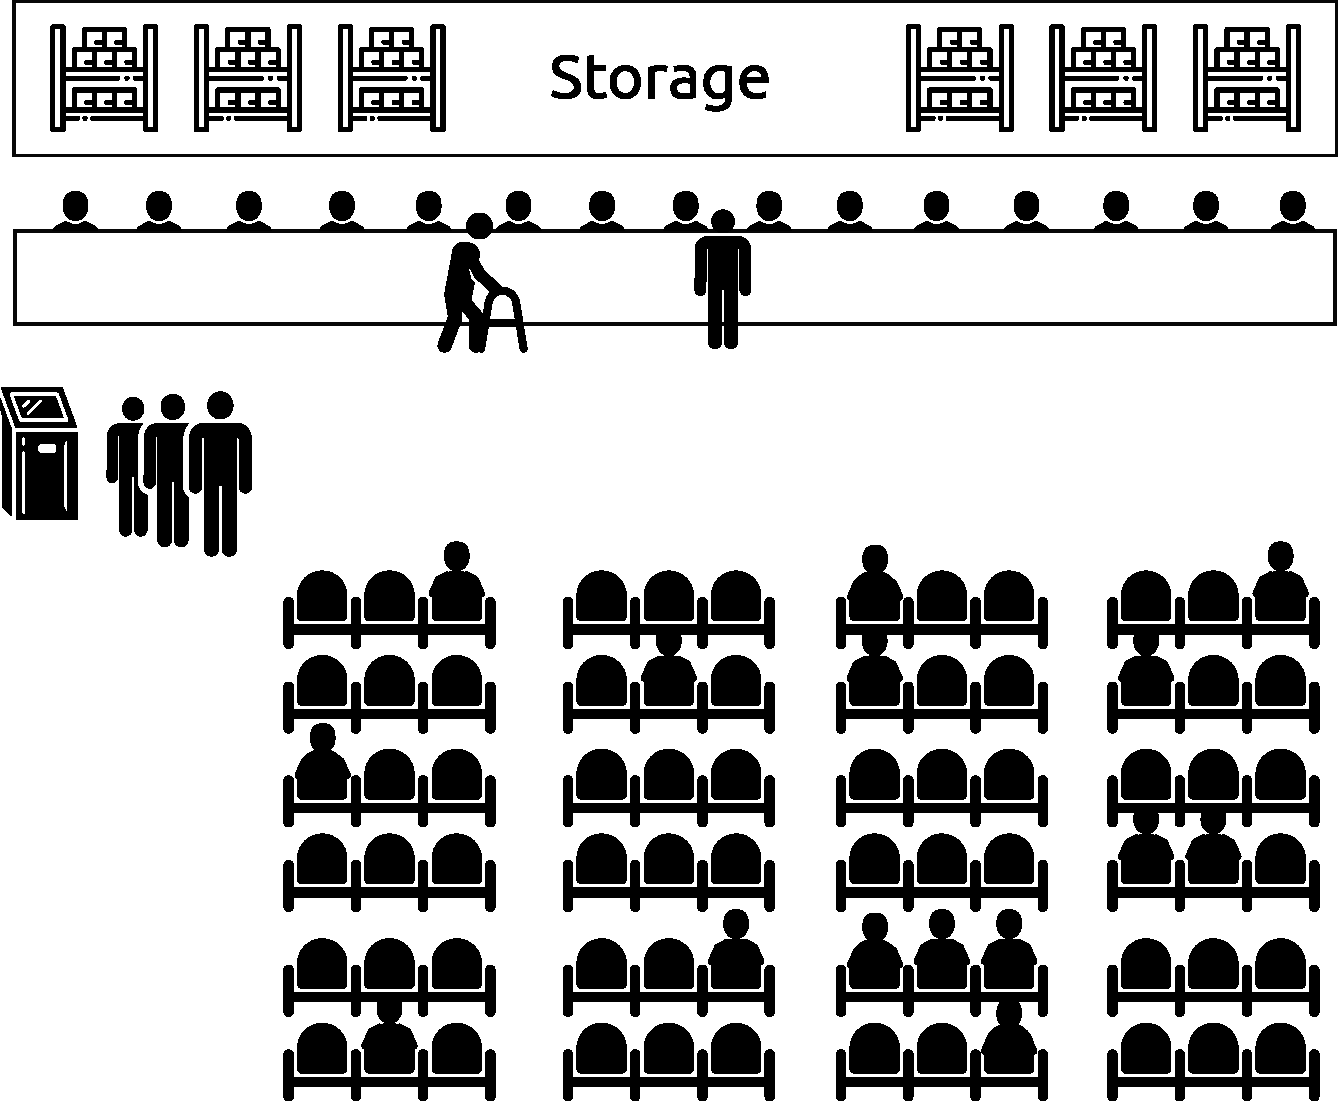
\includegraphics[scale=.4]{images/drawing.pdf}
    \end{figure}
\end{frame}
\section{WHY DES?}
\begin{frame}{WHY DES?}

\begin{multicols}{2}
\textbf{Real System Experimentation}\\
\cite{reynolds2011using}
\columnbreak
\begin{itemize}
    \item Time consuming.
    \item High costs.
    \item One experiment at once.
    \item Potential havoc.
    \item Irreversible changes. % Factory
\end{itemize}
\end{multicols}
\begin{multicols}{2}
\textbf{Discrete Event Simulation}
\columnbreak
\begin{itemize}
    \item Almost no cost.
    \item No disruption or risks.
    \item Multiple scenarios at once.
    \item Simple inclusion of randomness.
\end{itemize}
\end{multicols}
\end{frame}
\section{OBJECTIVES}
\begin{frame}{OBJECTIVES}
\textbf{General Objective}
    \begin{itemize}
        \item To determine the priorities of each module in order to reduce the queue time of patients.
    \end{itemize}
    \vspace{.5cm}
\textbf{Specific Objectives}
    \begin{itemize}
        \item To select the most appropriate data to be considered in the model.
        \item To apply statistical tests  to filtered data in order to contrast different hypothesis.
        \item To validate and verify the implemented model using the available data.
        \item To explore multiple feasible strategies for queue priorities in the modules.
    \end{itemize}
\end{frame}
\section{CONCEPTUAL MODELLING}
\begin{frame}{CONCEPTUAL MODELLING}
    \begin{multicols}{2}
    \textbf{Inputs}
    \begin{itemize}
        \item Number of modules with priority by hours.
        \item Queue logistics.
        \item Types of service.
    \end{itemize}
    \vspace{.5cm}
    \textbf{Outputs}
    \begin{itemize}
    \item Waiting time for each type of patient.
    \item Average time.
    \item Average number of patients waiting.
    \item Leisure time.
\end{itemize}
    \columnbreak
    
    \textbf{Parameters}
    \begin{itemize}
    \item Inter-arrival times.
    \item Duration of the attention.
    \item Inter-service times for each attendant.
    \item Probability of quitting.
    \item Type of services.
    \end{itemize}
    \vspace{1cm}
    \begin{tabular}{cc}
         &  \\
         & \\
         &
    \end{tabular}
    
    \end{multicols}
\end{frame}

\subsection{Assumptions \& Simplifications}
\begin{frame}{CONCEPTUAL MODELLING}
    \framesubtitle{Assumption \& Simplifications}
    \textbf{Assumptions}
    \begin{itemize}
    \item Always medicine available.
    \item No skippers.
    \item Available attendants $\rightarrow$ other priorities.
    \item No voluntary call of patients.
    \end{itemize}
    
    \vspace{0.5cm}
    \textbf{Simplifications}
    \begin{itemize}
    \item No second call.
    \item Quitters $\rightarrow$ constant probability.
    \item Data used $\rightarrow$ last week of August.
    \end{itemize}
    \end{frame}
\section{BACKGROUND}
\begin{frame}{BACKGROUND}
\begin{itemize}
    \item \cite{cobham1954priority} $\rightarrow$ Theoretical background priority queues.
    \item \cite{jun1999application}  and \cite{thorwarth2009application} $\rightarrow$ Review of DES in health care.
    \item \cite{lakshmi2013application} $\rightarrow$ Review of queue theory in health care.
    \item \cite{shimshak1981priority} and \cite{ndukwe2011reducing} $\rightarrow$ analysis of queue disciplines.
\end{itemize}
\vspace{0.5cm}
    \begin{figure}
        \centering
        \only<1>{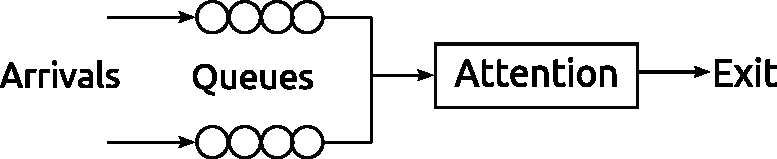
\includegraphics[scale=.5]{images/mult_queue_single_serv.pdf}}
        \only<2>{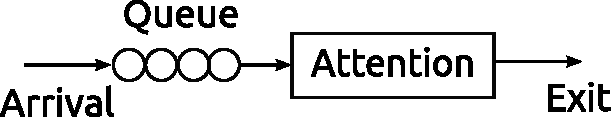
\includegraphics[scale=.5]{images/Signle_queue_s_server.pdf}}
        \only<3>{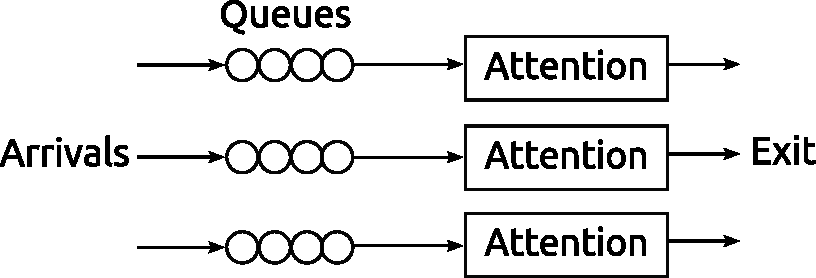
\includegraphics[scale=.5]{images/mult_queue_mult_serv.pdf}}
        \only<4>{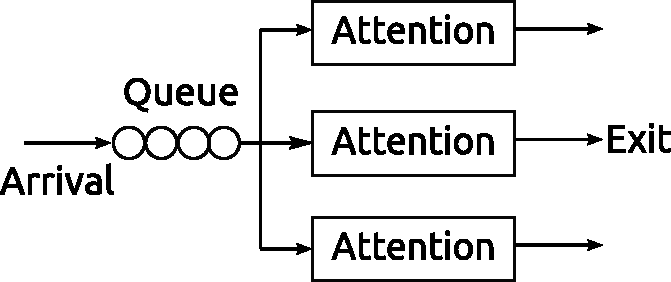
\includegraphics[scale=.5]{images/single_queue_mult_serv.pdf}}
    \end{figure}
\end{frame}
\section{MODEL DATA}
\subsection{Priority Data}
\begin{frame}{MODEL DATA}
\framesubtitle{Priority Data}
\begin{multicols}{2}
    \begin{table}[H]
    \centering
    \begin{tabular}{lp{4cm}}
    \hline
    \textbf{ID} & \textbf{Name}                                       \\ \hline
    3           & General Pharmacy                                    \\
    4           & Appointment confirmation \& PAC, MP and policy SURA \\
    5           & Procedure after appointment                                             \\
    7           & Preferential Pharmacy                               \\
    8           & Pharmacy PAC, MP y SURA policy                      \\
    9           & Preferential Appointment confirmation 
             \\
    10       & Scheduled retrieval    
    \\ \hline
    \end{tabular}
    \caption{Types of services}
    \label{tab:types_serv}
    \end{table}
    \columnbreak
    \begin{table}[H]
\centering
\begin{tabular}{ccl}
\hline
\textbf{Set} & \textbf{Amount} & \textbf{Priority} \\ \hline
1            & 1               & {[}10{]}          \\ 
2            & 1               & {[}4, 9, 5{]}     \\
3            & 1               & {[}4, 5, 9{]}     \\
4            & 2               & {[}7, 3, 8, 10{]} \\
5            & 4               & {[}3, 8, 7, 10{]} \\
6            & 5               & {[}3, 7, 8, 10{]} \\
\hline
\end{tabular}
\caption{Sets and priorities.}
\label{tab:sets_priorities_opt}
\end{table}

\end{multicols}
\end{frame}

\subsection{Distribution Fitting}
\begin{frame}{MODEL DATA}
    \framesubtitle{Distribution Fitting}
    \begin{itemize}
        \item Arrivals \& service times $\rightarrow$ Kolmogorov-Smirnov \citep[pp. 230-231]{banks2005discrete}
        \item Arrivals $\rightarrow$ Kruskal-Wallis \citep[pp. 765-767]{wackerly2010estadistica}.
    \end{itemize}
    \begin{figure}[H]
        \centering
        \begin{subfigure}[b]{0.475\textwidth}
            \centering
            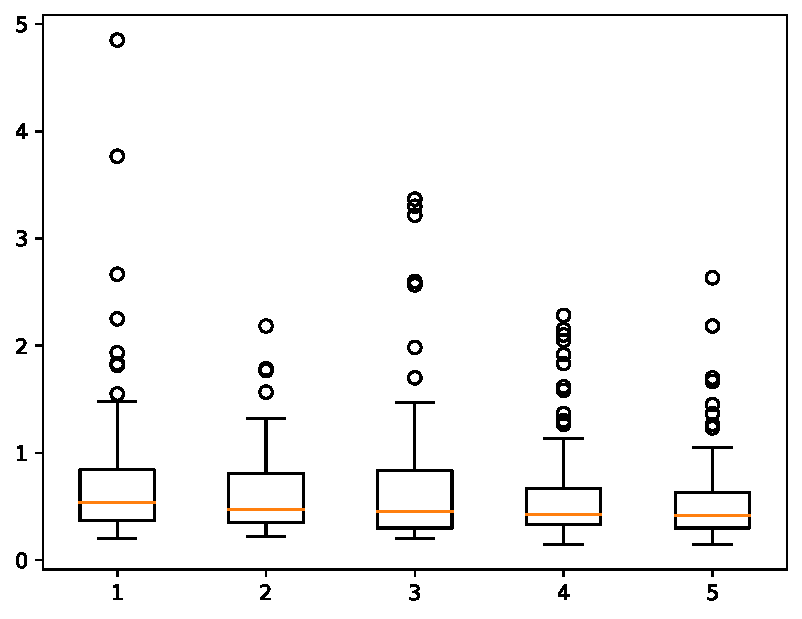
\includegraphics[scale=0.4]{images/homogeneity-test-for-thursday-hour-7.pdf}
            \caption{Boxplot.}
            \label{subfig:boxplot}
        \end{subfigure}
        \begin{subfigure}[b]{0.475\textwidth}   
            \centering 
            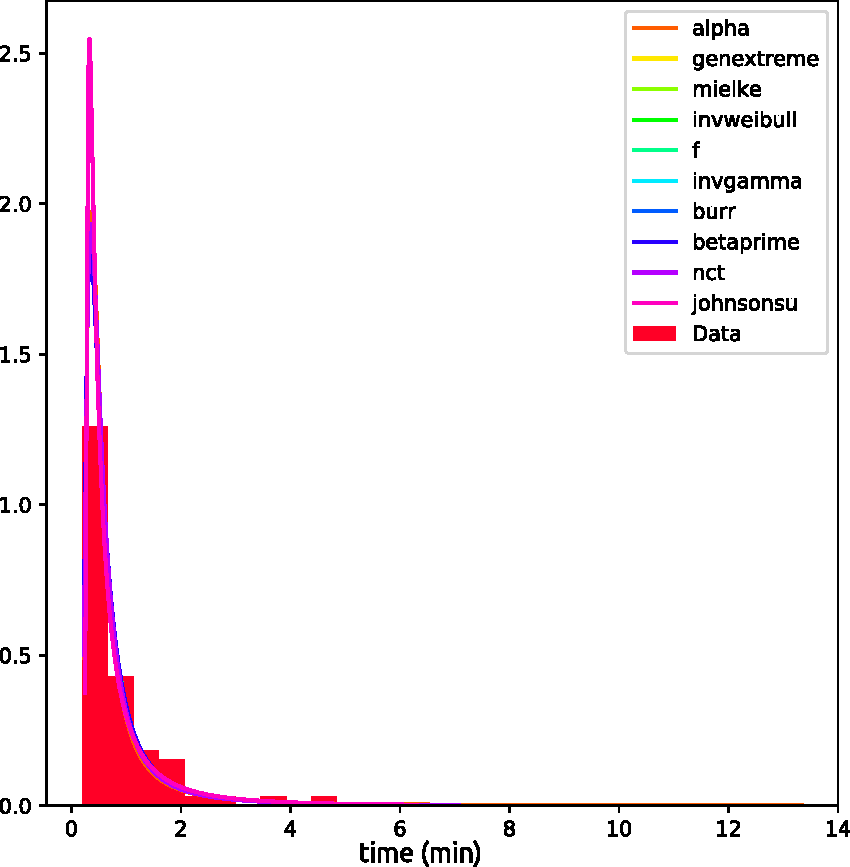
\includegraphics[scale=0.3]{images/fitting.pdf}
            \caption{Distribution fitting.}
            \label{subfig:dist}
        \end{subfigure}
        \caption{Data for Thursdays at 7 a.m.}
        \label{fig:thu7}
	\end{figure}
\end{frame}

\section{IMPLEMENTATION}
\begin{frame}{IMPLEMENTATION}
    \begin{figure}
        \centering
        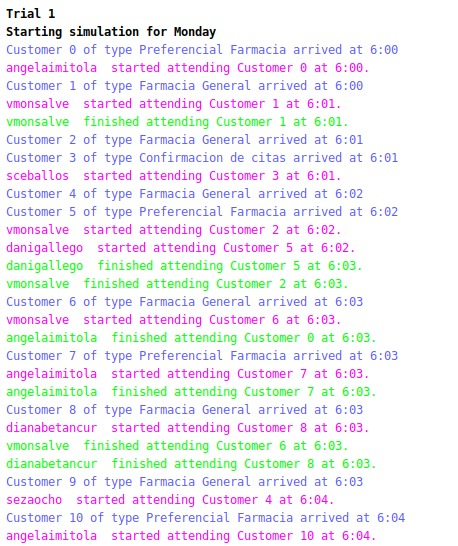
\includegraphics[scale=0.35]{images/model.jpeg}
        \caption{Model in execution.}
    \end{figure}
\end{frame}

\section{RESULTS}
\begin{frame}{RESULTS}
\begin{multicols}{2}
\begin{itemize}
    \item Nature of simulation $\rightarrow$ terminating.
    \item Output nature $\rightarrow$ transient.
    \item Biased $\rightarrow$ Not considered.
    \item Initial/final conditions $\rightarrow$ zero.
    \item Number of runs $\rightarrow$ huge.\\ 
\columnbreak
    \begin{equation*}
    n \geq\left(\frac{t_{\alpha/2;n_0-1} \times \sigma}{\delta}\right)^{2}
    \end{equation*}
\end{itemize}
\end{multicols}
\begin{figure}
    \centering
    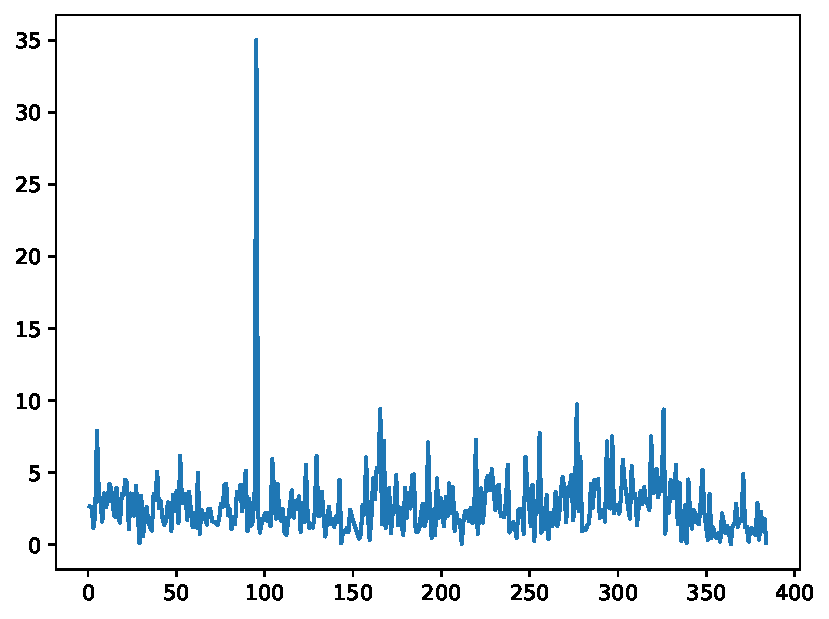
\includegraphics[scale=.4]{images/time-series.pdf}
    \caption{Time series for average waiting time in a week.}
\end{figure}
\end{frame}

\section{VERIFICATION \& VALIDATION}
\begin{frame}{VERIFICATION \& VALIDATION}
    \citep[Ch. 12]{robinson2004simulation}
    \begin{multicols}{2}
        \textbf{White-Box}
        \begin{itemize}
            \item Extreme conditions
            \item Initial conditions
            \item Distributions
            \item Priorities
        \end{itemize}
        \begin{figure}
            \centering
            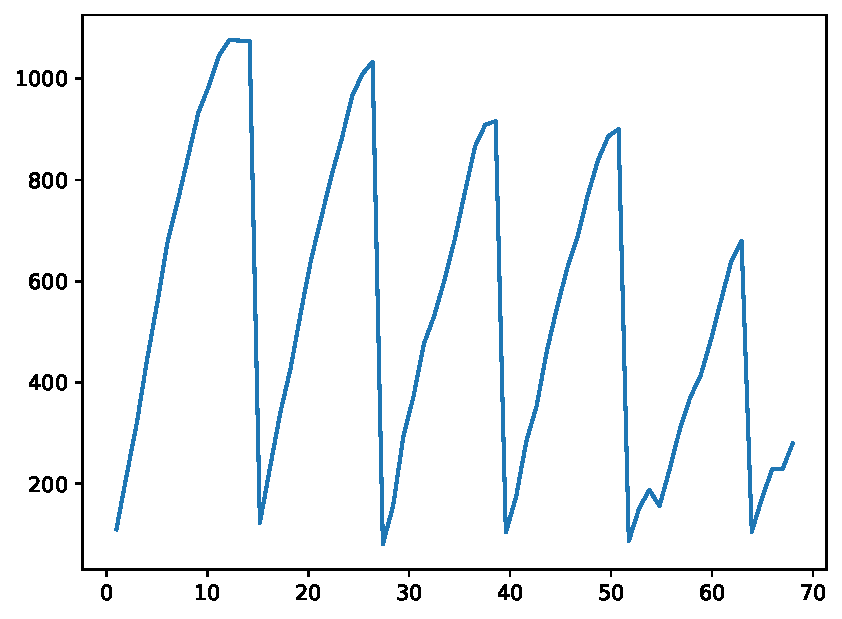
\includegraphics[scale=.35]{images/validation.pdf}
            \caption{Number of patients for each hour with one attendant.}
        \end{figure}
        \columnbreak
        \textbf{Black-Box}
        \begin{itemize}
            \item Confidence interval
        \end{itemize}
                
        \begin{equation*}
        \bar{X}_{\mathrm{S}}-\bar{X}_{R} \pm t_{\alpha / 2; 2 n-2} \sqrt{\frac{S_{S}^{2}+S_{R}^{2}}{n}}
        \end{equation*}
         \[[-55.71, -53.60]\]
    \end{multicols}
\end{frame}
\section{EXPERIMENTATION}
\subsection{Sensitivity Analysis}
\begin{frame}{EXPERIMENTATION}
    \framesubtitle{Sensitivity Analysis}
    \begin{itemize}
        \item Not enough data or rejected distributions $\rightarrow$ parameters or other distribution.
        \item Number of open modules.
    \end{itemize}
    \begin{figure}
        \centering
        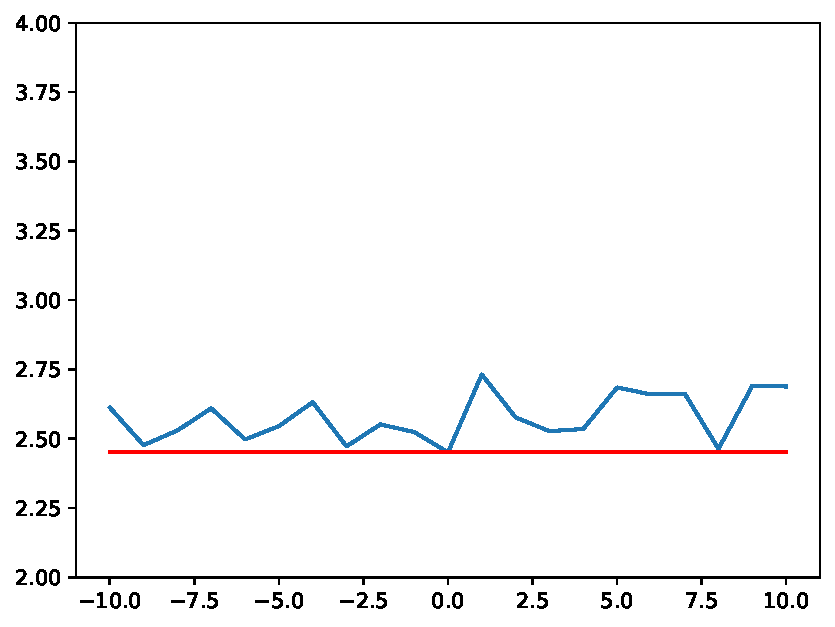
\includegraphics[scale=.5]{images/sensitivity.pdf}
        \caption{Sensitivity analysis $\pm$10\% in mean of assumed distributions.}
    \end{figure}
\end{frame}

\subsection{Optimization}
\begin{frame}{EXPERIMENTATION}
    \framesubtitle{Optimization}
    \begin{itemize}
        \item Minimize time in queue for each type of service.
        \item Best combination for priorities of Table \ref{tab:sets_priorities_opt}.
        \item Heuristic Approach $\rightarrow$ Local search $\rightarrow$ VNS.
    \end{itemize}
    \begin{multicols}{2}
    \begin{figure}
        \centering
        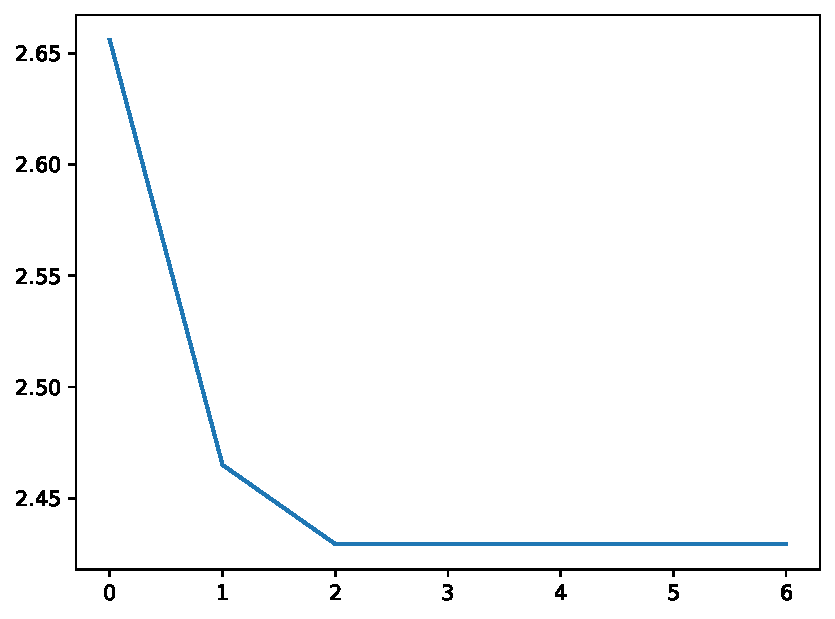
\includegraphics[scale=.4]{images/opti.pdf}
        \caption{Heuristic results}
    \end{figure}
    \columnbreak
    \begin{table}[H]
\centering
\begin{tabular}{cl}
\hline
\textbf{Set} & \textbf{Priority} \\ \hline
1            & {[}5, 4, 9{]}     \\
2            & {[}8, 10, 7, 3{]} \\
3            & {[}7, 3, 10, 8{]} \\
4            & {[}8, 10, 3, 7{]} \\
5            & {[}3, 7, 8, 10{]} \\
6            & {[}8, 3, 7, 10{]} \\ \hline
\end{tabular}
\caption{Sets and priorities.}
\label{tab:sets_priorities_opt}
\end{table}
    \end{multicols}
\end{frame}


\section{CONCLUSIONS}
It was successfully analyzed the received data, using statistical tests which allowed to fit data to use in the simulation, find auto-correlation and test homogeneity between data. It is important to remark that in the fitting of the data the distributions have a left bias as most of the times are positive and close to zero.

It was successfully implemented the simulation model in Python, which partially represents the Neuromédica pharmacy medicine retriveal system. The model did not fully validate with the tests done, which presents an important limitation of the implemented model; even though, the results given are not useful for the real system, this article proposes a methodology for solving this types of problems. 

For further work, a model using continuous simulation could be used as the inter-arrival times are so close to zero that the system could be analyzed supposing a continuous flux of patients. Also, a graphical user interface can be done so it is easily explained without the use of code.
\nonumb % Not numbered titles
%\addcontentsline{toc}{section}{\small\protect\numberline{}{REFERENCIAS BIBLIOGRÁFICAS}} % Separated from other contents, for small number of contents
\addcontentsline{toc}{section}{\small REFERENCES} % Closer from other contents, for large number of contents
\nocite{*} % All citations showed (take care with fraud!)
%%%%%%%%%%%%%%%%%%%%%%%%%%%%%%%%%%%%%%%%%%%%%%%%%%%%%%%%%%%%%%%%%%%%%%%%%%%%
\section*{REFERENCES}
\begin{frame}[allowframebreaks]{REFERENCES} %  and put before {REFEREN...}
\begingroup % Group for changing the color
\renewcommand{\color}[1]{} % Allows to have black bibs and white footnote bibs
\small{\bibliographystyle{IEEEtran}} % Size of text; acm or gatech-thesis or ieeetr or ieeetran or icontec or iso690
\bibliography{ref}
\endgroup % Group for changing the color
% pdflatex -> bibtex -> pdflatex -> pdflatex
\end{frame}
%%%%%%%%%%%%%%%%%%%%%%%%%%%%%%%%%%%%%%%%%%%%%%%%%%%%%%%%%%%%%%%%%%%%%%%%%%%%
% Thank-slide
\begin{frame}[plain,noframenumbering] % No frame number
	\begin{beamercolorbox}[ht=\paperheight,wd=\paperwidth, center]{Portada}
		\begin{center}\Huge\textbf{Thank you}\end{center} % Or Thanks; leave the next space mandatorily
		
		\vspace{0.44\paperheight}
    \end{beamercolorbox}
\end{frame}
%%%%%%%%%%%%%%%%%%%%%%%%%%%%%%%%%%%%%%%%%%%%%%%%%%%%%%%%%%%%%%%%%%%%%%%%%%%%


\end{document}